\section{Rachunek Gentzena}

\subsection{Wzory}

\begin{tabularx}{\textwidth}{X X X X}
    \centering
    $ \displaystyle\frac{\phi \rightarrow \neg \alpha ,\psi }{\phi, \alpha \rightarrow \psi} $ & 
    $ \displaystyle\frac{\phi \rightarrow \alpha \lor \beta, \psi }{\phi \rightarrow \alpha, \beta, \psi} $ &
    $ \displaystyle\frac{\phi \rightarrow \alpha \land \beta, \psi }{\phi, \alpha \rightarrow \psi || \phi, \beta \rightarrow \psi} $ &
    $ \displaystyle\frac{\phi \rightarrow \alpha, \alpha \psi}{\phi \rightarrow \alpha, \psi} $ \\[20pt]

    \centering
    $ \displaystyle\frac{\phi, \neg \alpha \rightarrow \psi}{\phi \rightarrow \alpha, \psi} $ &
    $ \displaystyle\frac{\phi, \alpha \lor \beta \rightarrow \psi}{\phi, \alpha \rightarrow \psi || \phi, \beta \rightarrow \psi} $ &
    $ \displaystyle\frac{\phi, \alpha \land \beta \rightarrow \psi}{\phi, \alpha, \beta \rightarrow \psi} $ & 
    $ \displaystyle\frac{\phi, \alpha, \alpha \rightarrow \psi}{\phi, \alpha \rightarrow \psi} $ \\[20pt]
\end{tabularx}

$ P_1 : (\alpha \Rightarrow \beta) \Leftrightarrow (\neg \alpha \lor \beta) \quad \quad 
P_2 : (\alpha \Leftrightarrow \beta) \Leftrightarrow ((\alpha \Rightarrow \beta) \land (\beta \Rightarrow \alpha)) $ \\

\textbf{Przykład}

$$ \rightarrow ((p \Rightarrow \neg q) \lor \neg(p \Rightarrow \neg q)) $$

Korzystając z praw rachunku zdań eliminujemy te funktory, których nie uwzględniliśmy w podanej liście przekształceń.

\pagebreak Schemat przyjmuje postać:

$$ \rightarrow ((\neg p \lor \neg q) \lor \neg(\neg p \lor \neg q)) $$
$$ \textrm{prawostronne} \ \lor $$
$$ \rightarrow (\neg p \lor \neg q), \ \neg(\neg p \lor \neg q) $$
$$ \textrm{prawostronne} \ \neg $$
$$ \neg p \lor \neg q \rightarrow \neg p \lor \neg q $$
$$ \textrm{prawostronne} \ \lor $$
$$ \neg p \lor \neg q \rightarrow \neg p, \neg q $$
$$ \lor \ \textrm{po lewej} $$

\renewcommand{\arraystretch}{1.4}

\begin{center}
\begin{tabularx}{\textwidth}{X>{\centering\arraybackslash} X}
    \centering
    $ \neg p \rightarrow \neg p, \neg q $ & $ \neg q \rightarrow \neg p, \neg q $ \\
    \centering
    $ 3 \times \neg $ & $ 3 \times \neg $ \\
    \centering
    $ q, \underline{p \rightarrow p} $ & $ p, \underline{q \rightarrow q} $ \\
    \centering
    Aksjomat & Aksjomat \\
\end{tabularx}
\end{center}

Z schematu wynika tautologia wtedy kiedy po lewej i po prawej stronie występuje ta sama zmienna np $ \alpha \rightarrow \alpha, \beta $

\begin{center}
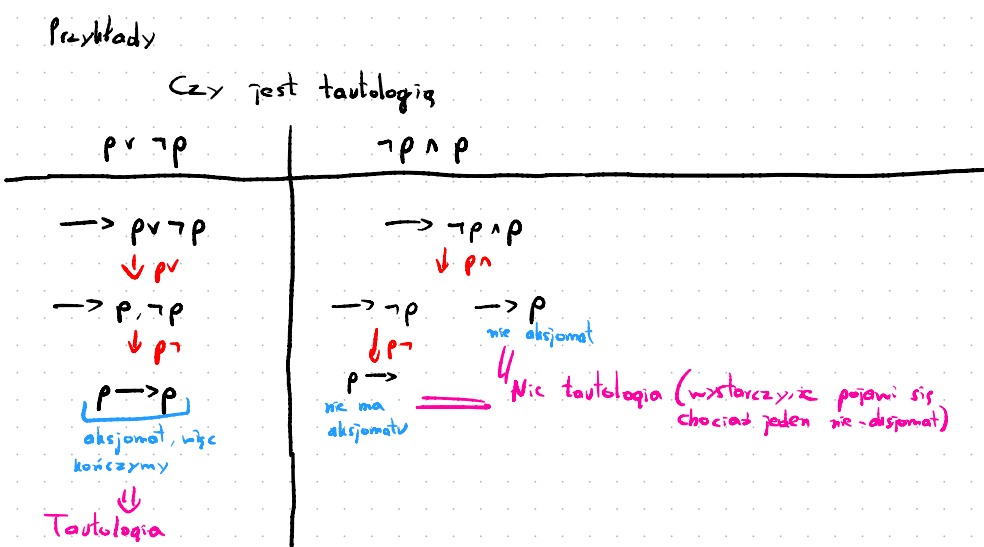
\includegraphics[scale=0.7]{img/gentzen.png}
\end{center}